%%\documentclass[12pt,letterpaper,doublespaced,ETD,dvips]{gt-ece-thesis}
\documentclass[12pt,letterpaper,doublespaced,ETD]{gt-ece-thesis} %taking dvips out enable pdf bookmark generation as well as the logo printing on the first page

\title{Target Tracking Using Residual Vector Quantization}
\author{Salman Aslam}
\copyrightyear{2011}
\graddate{20 June 2011}  
\approvaldate{June 2011}  

\addadvisor{Dr. Christopher F. Barnes}{Assoc. Professor, School of ECE}{Georgia Institute of Technology}
\addchair{Dr. David V. Anderson}{Assoc. Professor, School of ECE}{Georgia Institute of Technology}
\addreader{Dr. Aaron F. Bobick, Co-advisor}{Professor, School of Interactive Computing}{Georgia Institute of Technology}
\addreader{Dr. Vijay Madisetti}{Professor, School of ECE}{Georgia Institute of Technology}
\addreader{Dr. Patricio Vela}{Asst. Professor, School of ECE}{Georgia Institute of Technology}
\addreader{Dr. Santanu Dey}{Asst. Professor, School of ISYE}{Georgia Institute of Technology}


\bibfiles{f:/salman/work/writing/MyCitations}

\titlepagetrue
\figurespagetrue
\tablespagetrue
\contentspagetrue
\symbolspagefalse
\glossarypagefalse 
\bibpagetrue
\mastersthesisfalse 
\multivolumefalse
\singlespacednotestrue


\usepackage{graphicx, subfigure, verbatim}
\usepackage{insfig}
\usepackage{url}
\usepackage{multirow}
\usepackage{hyperref}
\usepackage{longtable}
\usepackage[usenames,dvipsnames]{color}
\definecolor{light-gray}{gray}{0.95}
\usepackage{amsmath,epsfig,verbatim,listings}
\lstset{breaklines=true,breakindent=0pt,
        prebreak=\mbox{\tiny$\searrow$},
        postbreak=\mbox{{\color{blue}\tiny$\rightarrow$}},
	tabsize=2,
linewidth=1.1\linewidth,
xleftmargin=-0.8in,
basicstyle=\tiny,
numbers=left,
frame=single,
captionpos=t,
title=\lstname,
backgroundcolor=\color{light-gray}}


\setchaptertocdepth{2}
\setappendixtocdepth{2}

\settocstring{Table of Contents}
\setlofstring{List of Figures}
%\setlotstring{List of Tables}
\setbibstring{References}
\setindstring{Index}
\setdedstring{Dedication}
\setglostring{List of Terms}
\setchpstring{Chapter}
\setappstring{Appendix}
\setprtstring{Volume}
\setabsstring{Summary}
\setlosstring{List of Symbols}
\setackstring{Acknowledgment}

\setfrontpagestyle{plain}
\setbodypagestyle{plain}
\setendpagestyle{plain}

\pagestyle{plain}
\bibliographystyle{ieeetr}
%\definecolor{darkgreen}{rgb}{0,0.5,0}
\newcommand{\Ntrg}{\big[N_{t=1, m=1} + \lambda \big] + \big[N_{t=1, m=2} + \lambda \big] + \ldots + \big[N_{t=1, m=M} + \lambda \big]}
\newcommand{\jointcnt}{\sum\limits_{n_{trg}=1}^{N_{trg}}I(X_t=x_t, X_{t-1}=x_{t-1})}
\newcommand{\singlecnt}{\sum\limits_{n_{trg}=1}^{N_{trg}}I(X_{t-1}=x_{t-1})}
\newcommand{\singlep}{p(X_{t-1}=x_{t-1})}
\newcommand{\singlepone}{p(X_{t-1}=1)}
\newcommand{\singleptwo}{p(X_{t-1}=2)}
\newcommand{\singlepM}{p(X_{t-1}=M)}
\newcommand{\condp}{p(X_t=x_t | X_{t-1}=x_{t-1})}
\newcommand{\jointp}{p(X_t=x_t, X_{t-1}=x_{t-1})}
\newcommand{\KmeansOuterSum}{\sum\limits_{k=1}^K}
\newcommand{\KmeansInnerSum}{\sum\limits_{{i=1 \atop x_i \in \mathcal{K}_k}}^N}
\newcommand{\KmeansSum}{\KmeansOuterSum \KmeansInnerSum}
\newcommand{\RVQInnerSum}{\sum\limits_{{i=1 \atop g_i \mapsto m_{\tau, s}}}^N}
\newcommand{\RVQOuterSum}{\sum_{s=1}^S}
\newcommand{\RVQsum}{\KmeansOuterSum \sum\limits_{{i=1 \atop g_i \in \mathcal{K}_k}}^N}
\newcommand{\KmeansInner}{{(x_i - \mu_k)}^2}
\newcommand{\RVQinner}{            {(x_i  - \hat{\mu}^{(k)})}^2}
\newcommand{\RVQinneralternate}{{(g_i - m_\tau^{(k)})}^2}
\newcommand{\RVQinneralternatealternate}{{(g_i - m_{\tau, s})}^2}
\newcommand{\KmeansError}{\KmeansSum \KmeansInner}
\newcommand{\RVQerror}     {\KmeansSum \RVQinner}
\newcommand{\RVQerroralternate}{\RVQsum \RVQinneralternate}
\newcommand{\RVQunit}{x_i -\bigg(\sum_{t=1}^Tm^{(k)}_t\bigg)}
\newcommand{\RVQequivalentCodevector}{\sum_{t=1 }^Tm^{(k)}_t}
\newcommand{\RVQequivalentCodevectorBroken}{\sum_{t=1 \atop t \neq \tau}^Tm^{(k)}_t+ m^{(k)}_\tau}
\newcommand{\RVQmultipleKmeans}{x_i -\bigg(\RVQequivalentCodevectorBroken\bigg)}
\newcommand{\RVQmultipleKmeansone}{x_i -\sum_{t=2}^Tm^{(k)}_t+ m^{(k)}_1\bigg)}
\newcommand{\RVQmultipleKmeansonealternate}{\bigg(x_i -\sum_{t=1 \atop t \neq \tau}^Tm^{(k)}_t\bigg) - m^{(k)}_\tau}
\newcommand{\RVQmultipleKmeanstwo}{x_i -\bigg(\sum_{t=1 \atop t \neq 2}^Tm^{(k)}_t+ m^{(k)}_2\bigg)}
\newcommand{\RVQmultipleKmeansT}{x_i -\bigg(\sum_{t=1}^{T-1}m^{(k)}_t+ m^{(k)}_2\bigg)}
\newcommand{\EucMatrix}
{
\left[
\begin{array}{lll}
r_{11} & r_{12} & t_x \\ 
r_{21} & r_{22} & t_y \\ 
0 & 0 & 1 \\ 
\end{array}
\right]
}	

\newcommand{\SimMatrix}
{
\left[
\begin{array}{lll}
sr_{11} & sr_{12} & t_x \\ 
sr_{21} & sr_{22} & t_y \\
0 & 0 & 1 \\ 
\end{array}
\right]
}

\newcommand{\AffMatrix}
{
\left[
\begin{array}{lll}
a &b & t_x \\ 
c & d & t_y \\
0 & 0 & 1 \\
\end{array}
\right]
}

\newcommand{\ProjMatrix}
{
\left[
\begin{array}{lll}
h_{11} & h_{12} & h_{13} \\ 
h_{21} & h_{22} & h_{23} \\ 
h_{31} & h_{32} & h_{33} \\ 
\end{array}
\right]
}

\newcommand{\RotMatrixTheta}
{
\left[
\begin{array}{rr}
\cos(\theta) & -\sin(\theta) \\ 
\sin(\theta) & \cos(\theta) \\ 
\end{array}
\right]
}

\newcommand{\RotMatrixPhi}
{
\left[
\begin{array}{rr}
\cos(\phi) & -\sin(\phi) \\ 
\sin(\phi) & \cos(\phi) \\ 
\end{array}
\right]
}

\newcommand{\RotMatrixminusPhi}
{
\left[
\begin{array}{rr}
\cos(-\phi) & -\sin(-\phi) \\ 
\sin(-\phi) & \cos(-\phi) \\ 
\end{array}
\right]
}


\newcommand{\EigenvalueMatrix}
{
\left[
\begin{array}{cc}
\lambda_1 & 0\\
0 & \lambda_2
\end{array}
\right]
}

\newcommand{\bigMatrix}
{
s \left[
\begin{array}{cc}
 (r)(a) + b &  (r)(d) - c \\
 (r)(c) - d &  (r)(b) + a
\end{array}
\right]
}


\newcommand{\bigMatrixTwo}
{
\left[
\begin{array}{cc}
(\lambda_2) p + (\lambda_1) q & (\lambda_2) s  - (\lambda_1) r \\
(\lambda_2) r  - (\lambda_1) s & (\lambda_2) q + (\lambda_1) p
\end{array}
\right]
}
\newcommand{\dr}{(\mathbf{x}_i-\boldsymbol\mu_k)^T(\mathbf{x}_i-\boldsymbol\mu_k) + \lambda({Q_{\textrm{max}}-Q_i})}

%\begin{document}
%\begin{FrontMatter}
%\contents %generates the TOC, LOF, and LOT
%\end{FrontMatter}
%\begin{Body}

%@@@@@@@@@@@@@@@@@@@@@@@@@@@@@@@@@@@@@@@@@@@@@@@@@@
\chapter{Results}
\label{chap_results}	
%@@@@@@@@@@@@@@@@@@@@@@@@@@@@@@@@@@@@@@@@@@@@@@@@@@


\begin{table}[t]
\footnotesize
\begin{tabular}{p{0.6in}|p{0.6in}p{0.6in}p{0.4in}p{0.4in}cccccc}
Dataset 		&Scenario	     &\parbox[c]{0.4in}{\center Time of \\day} 	&\parbox[c]{0.26in}{\center Target of \\interest}  &\parbox{0.3in}{\center Rigid \\target} 	&\parbox{0.4in}{\center Lighting change 1-5 \\(5 most severe)}  	&\parbox{0.5in}{\center Structured \\noise} 	&\parbox{0.4in}{\center Camera \\motion} 	&\parbox{0.3in}{\center Pose \\change} 	&\parbox{0.45in}{\center Expression \\change} 	&\parbox{0.3in}{\center Temporary \\occlusion} 	\\\hline
Dudek 		&Indoors		&N/A 				&face 		&no 	&2 	&yes 	&yes 	&yes 	&yes 	&yes 		\\\hline
davidin300 	&Indoors		&N/A				&face			&no	&3		&yes	&yes	&yes	&yes	&no		\\\hline
sylv			&Indoors		&N/A				&toy			&yes	&2		&no	&yes	&yes	&N/A	&no		\\\hline
fish			&Indoors		&N/A				&object		&yes	&5		&no	&yes	&no	&N/A	&no		\\\hline
car4			&Outdoors 	&day, sunny		&vehicle		&yes	&2		&no	&yes	&yes	&N/A	&no		\\\hline
car11			&Outdoors	&night			&vehicle		&yes	&1		&no	&yes	&yes	&N/A	&no		\\\hline
\end{tabular}
\caption{Datasets used for RVQ tracking.}
\label{Tab:datasets_used}
\end{table}


								\begin{figure}[t]
								\centering
								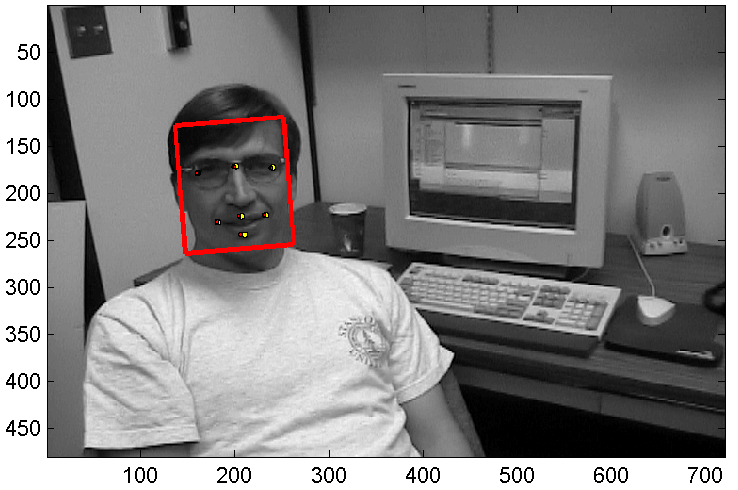
\includegraphics[width=0.7\textwidth]{thesis/results_pca__trk_dudek_0007.png}
								\caption{Computing tracking error.  The larger yellow circles indicate ground truth feature points.  The smaller red circles indicate estimated feature points.  Tracking error is computed using the rms error between the ground truth feature points and the estimated feature points.  In this particular frame, the tracking error is 2.57.}
								\label{fig:results_pca__trk_dudek_0007}
								\end{figure}

								\begin{figure}[t]
								\centering
								\begin{tabular}{|l|c|c|c|c|c|c|}
\hline
&\textbf{PCA}&\textbf{TSVQ}&\textbf{maxP}&\textbf{RofE}&\textbf{nulE}&\textbf{monR}\\\hline
\textbf{Dudek}&7.44&8.62&7.78&7.11&7.97&8.73\\\hline
\textbf{davidin300}&4.60&5.93&4.47&5.74&4.63&4.15\\\hline
\textbf{sylv}&4.34&4.61&4.00&4.12&4.74&4.31\\\hline
\textbf{fish}&2.17&4.59&2.78&2.73&2.48&2.89\\\hline
\textbf{car4}&4.60&5.11&4.67&4.93&5.28&4.71\\\hline
\textbf{car11}&2.13&2.21&2.17&2.33&2.52&2.47\\\hline
\textbf{ \% best}&50.00&0.00&16.67&16.67&0.00&16.67\\\hline
\end{tabular}

								\subfigure[Best tracking error for each algorithm.]{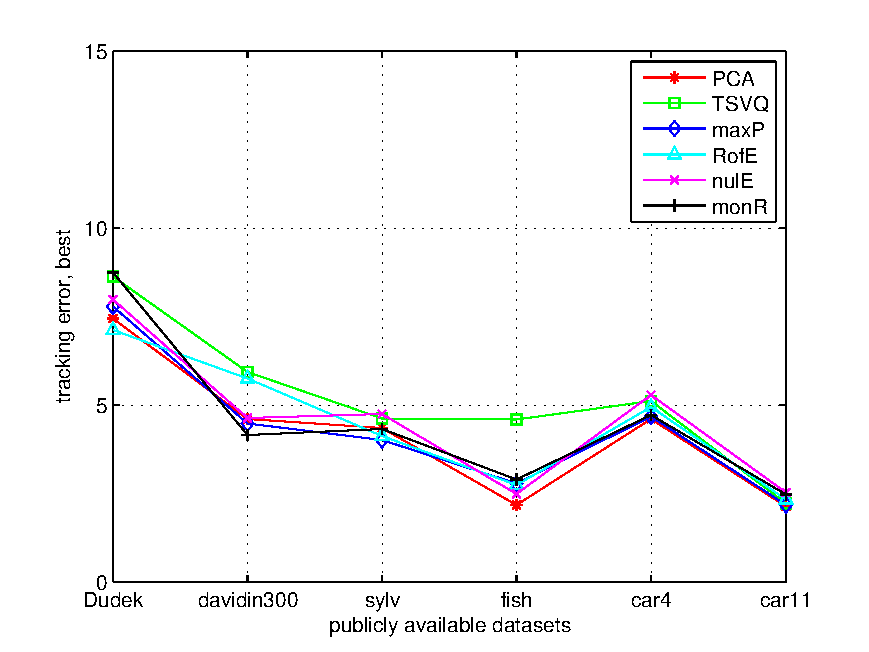
\includegraphics[width=0.47\textwidth]{thesis/results_final_1a_best.pdf}\label{fig:results_final_1a_best}}
								\subfigure[\%age of datasets over which best tracking error is achieved over all parameters.]{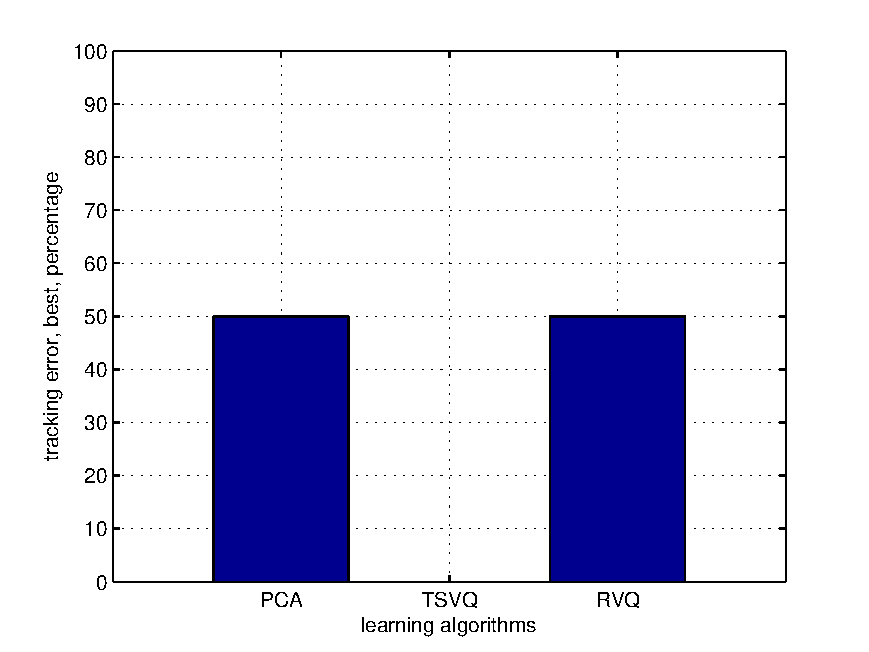
\includegraphics[width=0.47\textwidth]{thesis/results_final_1b_best_percent.pdf}\label{fig:results_final_1b_best_percent}}
								\caption{Tracking results (1 of 5), comparison of best tracking performance.  PCA give best performance for half the datasets, i.e. 3 datasets, while RVQ gives best performance for the other half.}
								\label{fig:results_final_1_best}
								\end{figure}

								\begin{figure}[t]
								\centering
								\begin{tabular}{|l|c|c|c|c|c|c|}
\hline
&\textbf{PCA}&\textbf{TSVQ}&\textbf{maxP}&\textbf{RofE}&\textbf{nulE}&\textbf{monR}\\\hline
\textbf{Dudek}&7.93&10.07&7.93&7.91&8.60&9.90\\\hline
\textbf{davidin300}&6.63&8.37&7.07&6.99&5.72&4.99\\\hline
\textbf{sylv}&5.18&4.70&4.47&4.83&5.10&4.66\\\hline
\textbf{fish}&6.63&6.71&8.81&5.97&5.74&6.15\\\hline
\textbf{car4}&4.97&5.90&5.38&5.19&5.77&4.99\\\hline
\textbf{car11}&2.24&3.48&2.70&2.49&2.69&2.58\\\hline
\textbf{ \% best}&33.33&0.00&16.67&16.67&16.67&16.67\\\hline
\end{tabular}

								\subfigure[Mean tracking error for each algorithm.]{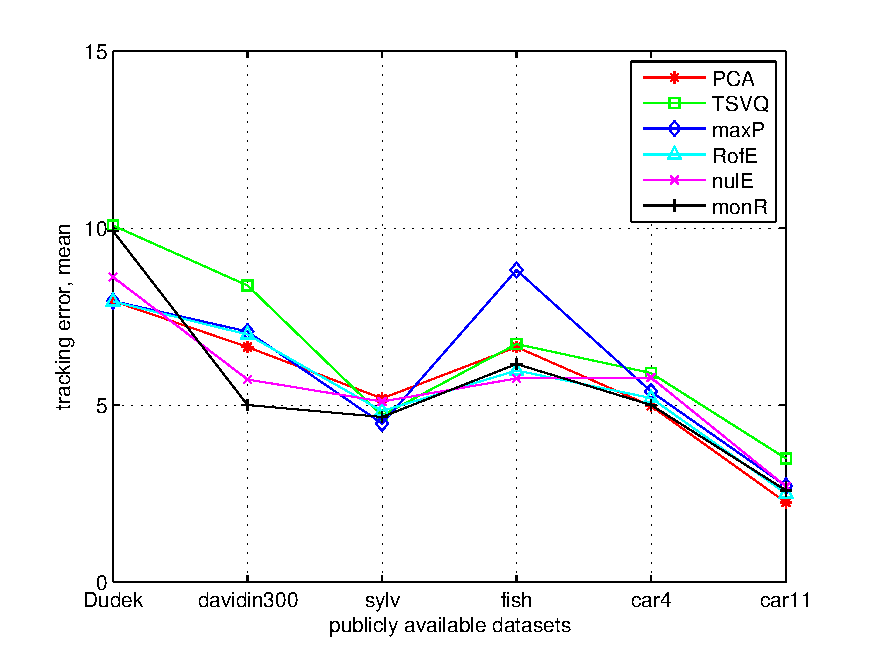
\includegraphics[width=0.47\textwidth]{thesis/results_final_2a_mean.pdf}\label{fig:results_final_2a_mean}}
								\subfigure[\%age of datasets over which best mean tracking error is achieved over all parameters.]{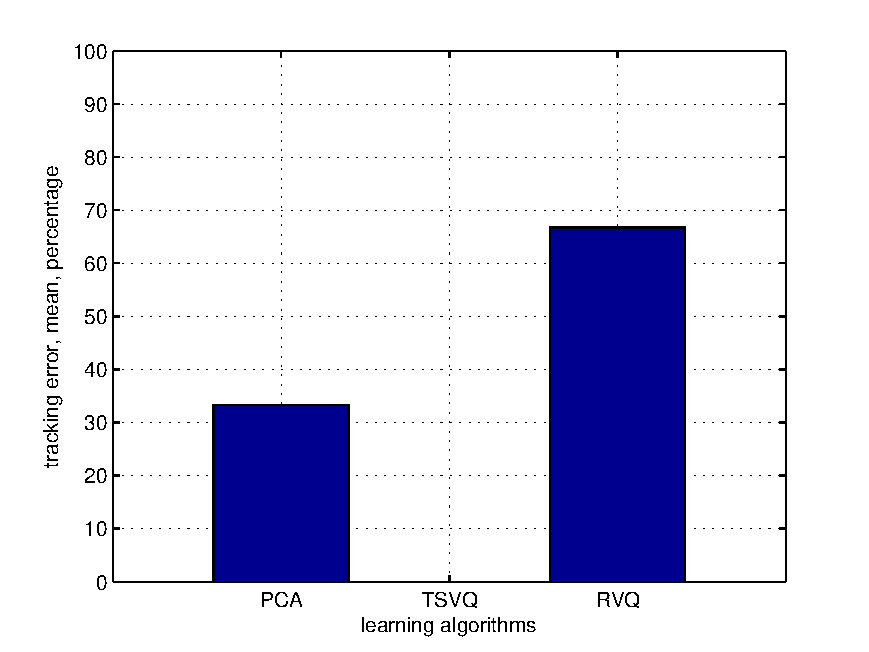
\includegraphics[width=0.47\textwidth]{thesis/results_final_2b_mean_percent.pdf}\label{fig:results_final_2b_mean_percent}}
								\caption{Tracking results (2 of 5), comparison of mean tracking performance.  RVQ performs better over twice as many datasets as PCA.}
								\label{fig:results_final_2_mean}
								\end{figure}

								\begin{figure}[t]
								\centering
								\begin{tabular}{|l|c|c|c|c|c|c|}
\hline
&\textbf{PCA}&\textbf{TSVQ}&\textbf{maxP}&\textbf{RofE}&\textbf{nulE}&\textbf{monR}\\\hline
\textbf{Dudek}&7.81&8.62&7.78&7.11&9.65&11.81\\\hline
\textbf{davidin300}&4.60&12.88&6.84&9.02&7.17&50.00\\\hline
\textbf{sylv}&5.47&4.70&4.00&4.12&4.81&4.31\\\hline
\textbf{fish}&2.17&10.07&11.50&2.96&4.03&2.89\\\hline
\textbf{car4}&4.60&5.11&4.67&4.93&5.28&5.07\\\hline
\textbf{car11}&2.13&2.21&2.17&2.47&2.59&2.47\\\hline
\textbf{ \% best}&66.67&0.00&16.67&16.67&0.00&0.00\\\hline
\end{tabular}

								\subfigure[Tracking error for each algorithm with 16 eigenvectors/code-vectors stored in memory.]{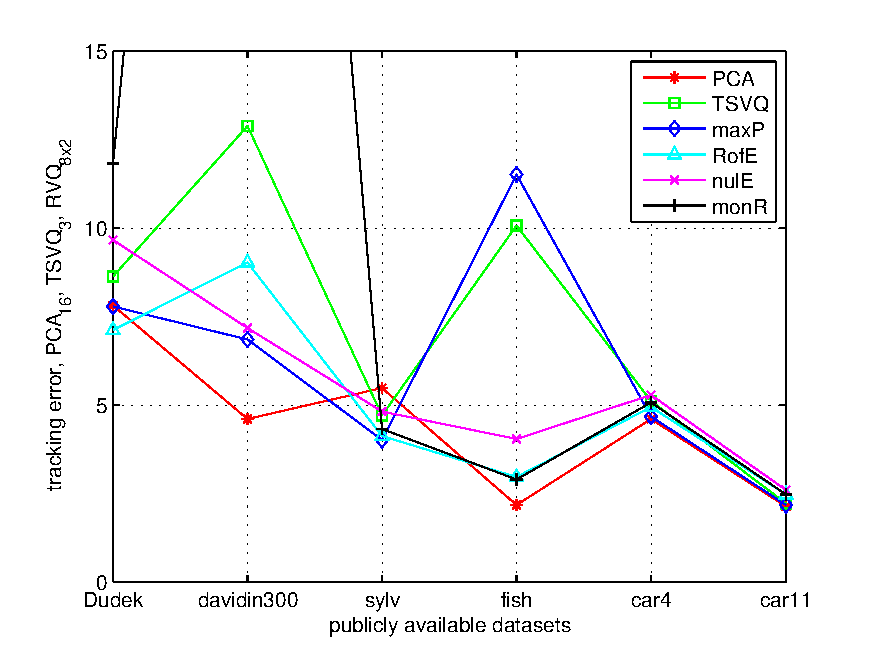
\includegraphics[width=0.47\textwidth]{thesis/results_final_3a_16.pdf}\label{fig:results_final_3a_16}}
								\subfigure[\%age of datasets over which best tracking error is achieved with 16 eigenvectors/code-vectors stored in memory.]{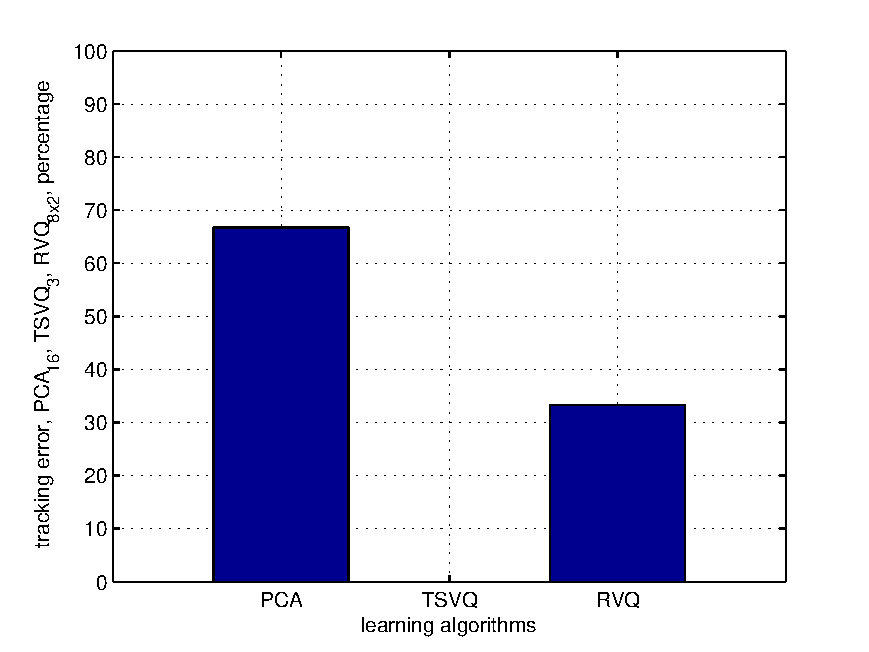
\includegraphics[width=0.47\textwidth]{thesis/results_final_3b_16_percent.pdf}\label{fig:results_final_3b_16_percent}}
								\caption{Tracking results (3 of 5), comparison of tracking performance if 16 eigenvectors/code-vectors are stored in memory.  PCA performs better over twice as many datasets as RVQ.}
								\label{fig:results_final_3_16}
								\end{figure}

								\begin{figure}[t]
								\centering
								\begin{tabular}{|l|c|c|c|c|c|c|}
\hline
&\textbf{PCA}&\textbf{TSVQ}&\textbf{maxP}&\textbf{RofE}&\textbf{nulE}&\textbf{monR}\\\hline
\textbf{Dudek}&8.54&11.87&7.92&8.43&8.19&9.17\\\hline
\textbf{davidin300}&6.93&6.29&4.47&6.21&5.35&5.83\\\hline
\textbf{sylv}&5.72&4.80&4.68&5.54&5.74&4.58\\\hline
\textbf{fish}&7.98&4.59&2.78&12.22&2.48&3.62\\\hline
\textbf{car4}&5.52&6.79&6.38&5.14&5.84&5.18\\\hline
\textbf{car11}&2.39&5.28&2.36&2.33&2.52&2.72\\\hline
\textbf{ \% best}&0.00&0.00&33.33&33.33&16.67&16.67\\\hline
\end{tabular}

								\subfigure[Tracking error for each algorithm with 32 eigenvectors/code-vectors stored in memory.]{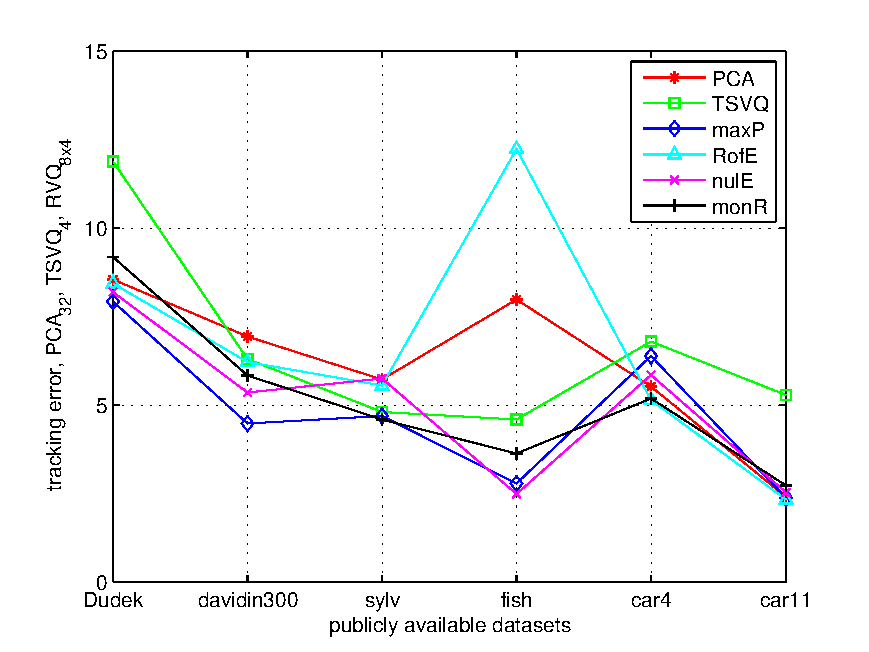
\includegraphics[width=0.47\textwidth]{thesis/results_final_4a_32.pdf}\label{fig:results_final_4a_32}}
								\subfigure[\%age of datasets over which best tracking error is achieved with 32 eigenvectors/code-vectors stored in memory.]{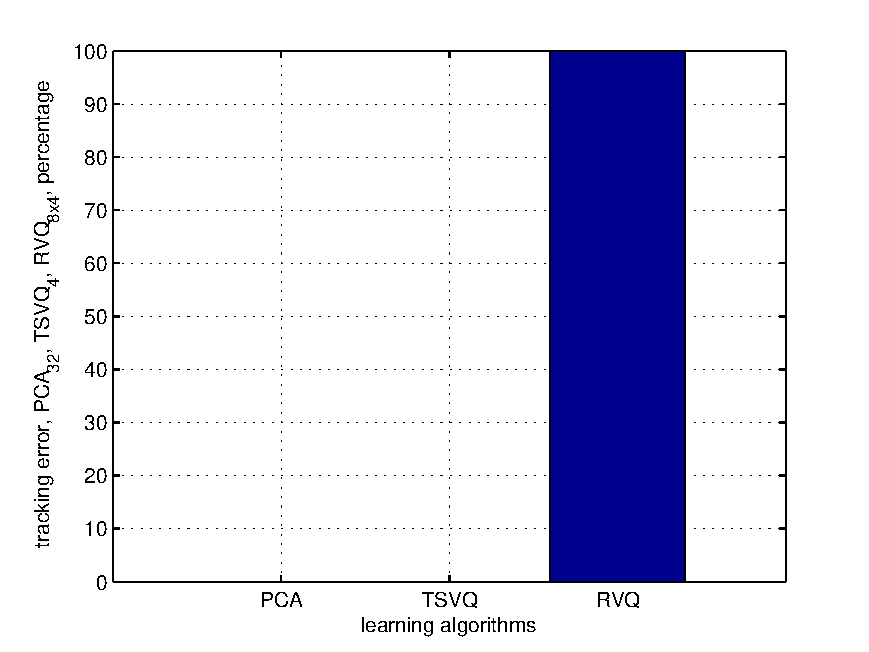
\includegraphics[width=0.47\textwidth]{thesis/results_final_4b_32_percent.pdf}\label{fig:results_final_4b_32_percent}}
								\caption{Tracking results (4 of 5), comparison of tracking performance if 32 eigenvectors/code-vectors are stored in memory.  RVQ performs the best over all datasets.}
								\label{fig:results_final_4_32}
								\end{figure}

								\begin{figure}[h!]
								\centering	
								\subtable[PCA.]{\begin{tabular}{|c|c|c|c|}
\hline
\textbf{8}&\textbf{16}&\textbf{32}&\textbf{mean}\\\hline
6.15&4.46&6.18&5.60\\\hline
\end{tabular}
}
								\subtable[TSVQ.]{\begin{tabular}{|c|c|c|c|}
\hline
\textbf{3}&\textbf{4}&\textbf{5}&\textbf{mean}\\\hline
7.26&6.60&5.74&6.54\\\hline
\end{tabular}
}
								\subtable[maxP.]{\begin{tabular}{|c|c|c|c|}
\hline
\textbf{8x2}&\textbf{8x4}&\textbf{8x8}&\textbf{mean}\\\hline
6.16&4.76&7.25&6.06\\\hline
\end{tabular}
}
								\subtable[RofE.]{\begin{tabular}{|c|c|c|c|}
\hline
\textbf{8x2}&\textbf{8x4}&\textbf{8x8}&\textbf{mean}\\\hline
5.10&6.64&4.94&5.56\\\hline
\end{tabular}
}
								\subtable[nulE.]{\begin{tabular}{|c|c|c|c|}
\hline
\textbf{8x2}&\textbf{8x4}&\textbf{8x8}&\textbf{mean}\\\hline
5.59&5.02&6.20&5.60\\\hline
\end{tabular}
}
								\subtable[monR.]{\begin{tabular}{|c|c|c|c|}
\hline
\textbf{8x2}&\textbf{8x4}&\textbf{8x8}&\textbf{mean}\\\hline
5.31&5.18&6.19&5.56\\\hline
\end{tabular}
}
								\subtable[maxP, RofE, nulE, monR.]{\begin{tabular}{|c|c|c|}
\hline
\textbf{8x2}&\textbf{8x4}&\textbf{8x8}\\\hline
5.54&5.40&6.15\\\hline
\end{tabular}
}\\
								\subfigure[PCA]{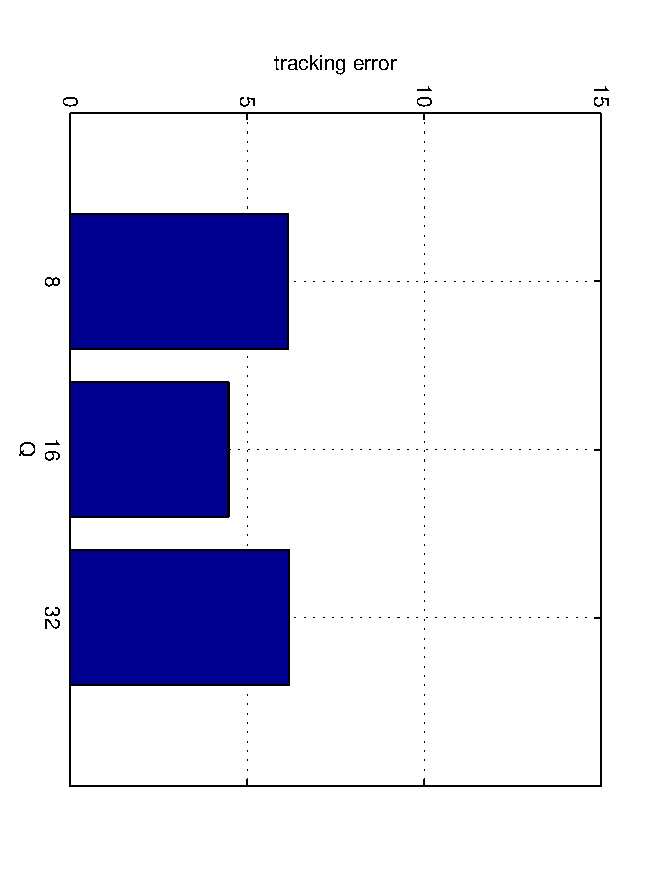
\includegraphics[width=0.225\textwidth, angle=90]{thesis/results_final_5a_pca_.pdf}\label{fig:results_final_5a_pca_}}
								\subfigure[TSVQ.]{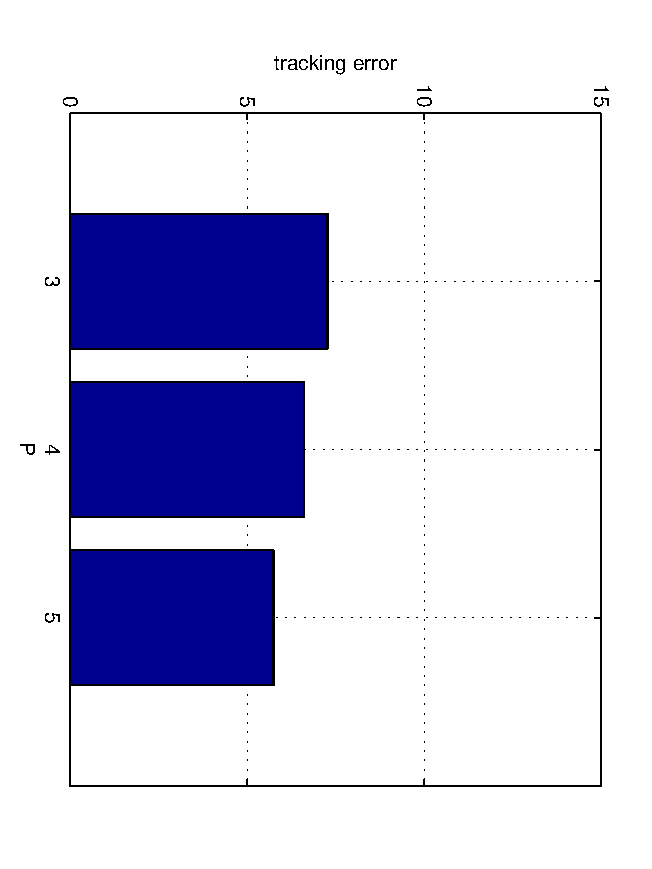
\includegraphics[width=0.225\textwidth, angle=90]{thesis/results_final_5b_tsvq.pdf}\label{fig:results_final_5b}}
								\subfigure[maxP.]{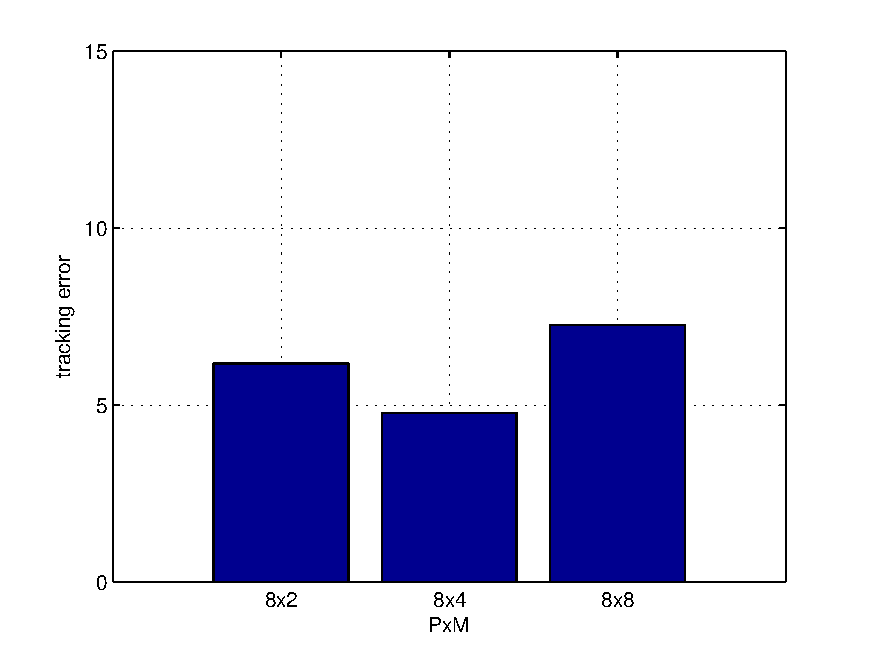
\includegraphics[width=0.3\textwidth]{thesis/results_final_5c_maxP.pdf}\label{fig:results_final_5c}}
								\subfigure[RofE.]{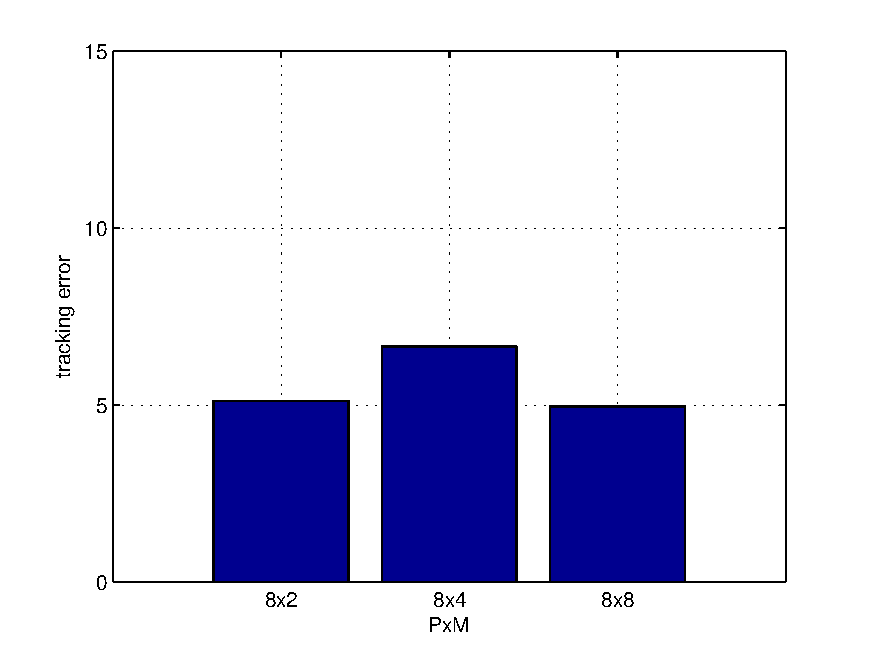
\includegraphics[width=0.3\textwidth]{thesis/results_final_5d_RofE.pdf}\label{fig:results_final_5d}}
								\subfigure[nulE.]{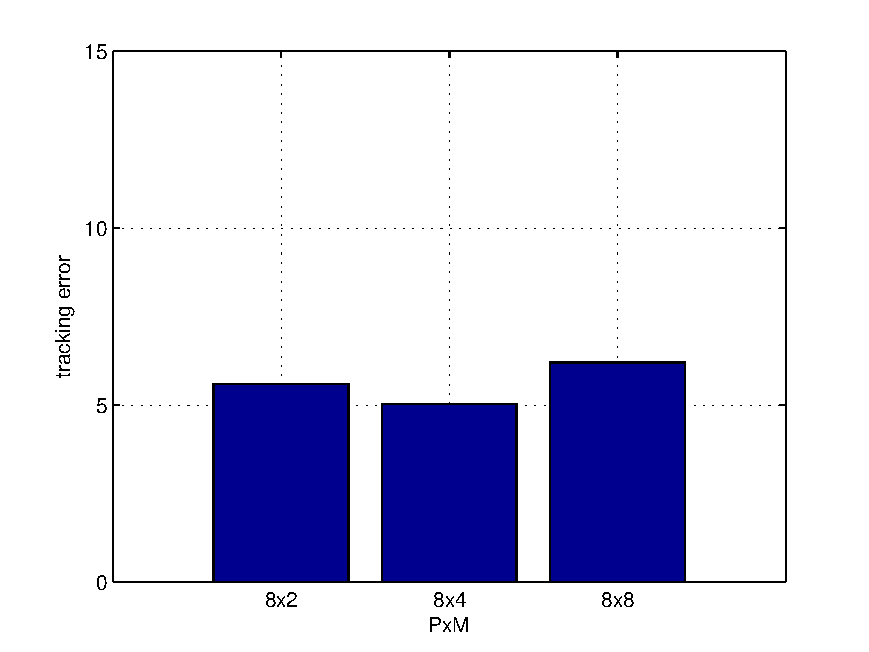
\includegraphics[width=0.3\textwidth]{thesis/results_final_5e_nulE.pdf}\label{fig:results_final_5e}}
							\subfigure[monR.]{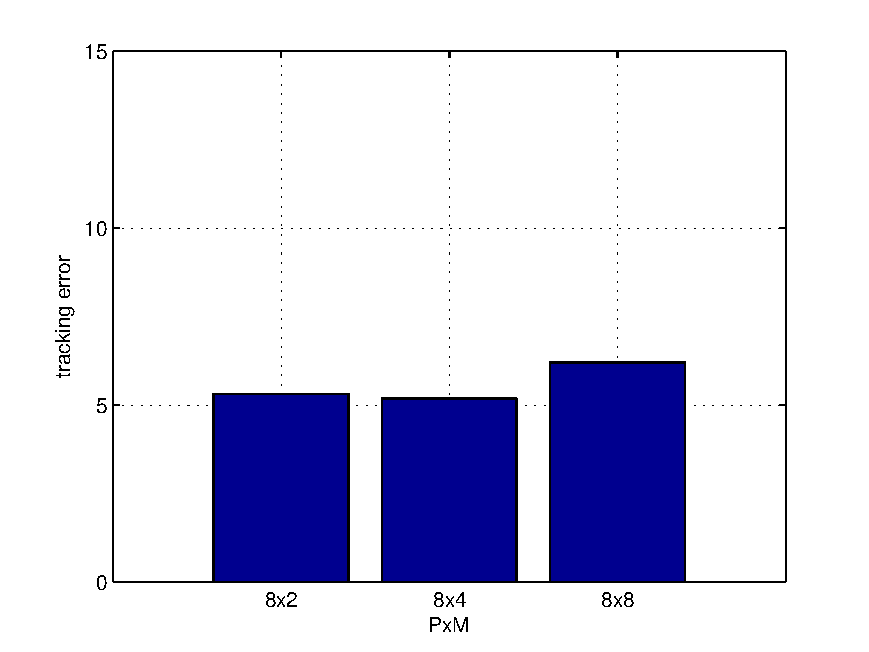
\includegraphics[width=0.3\textwidth]{thesis/results_final_5f_monR.pdf}\label{fig:results_final_5f}}
								\subfigure[maxP, RofE, nulE, monR.]{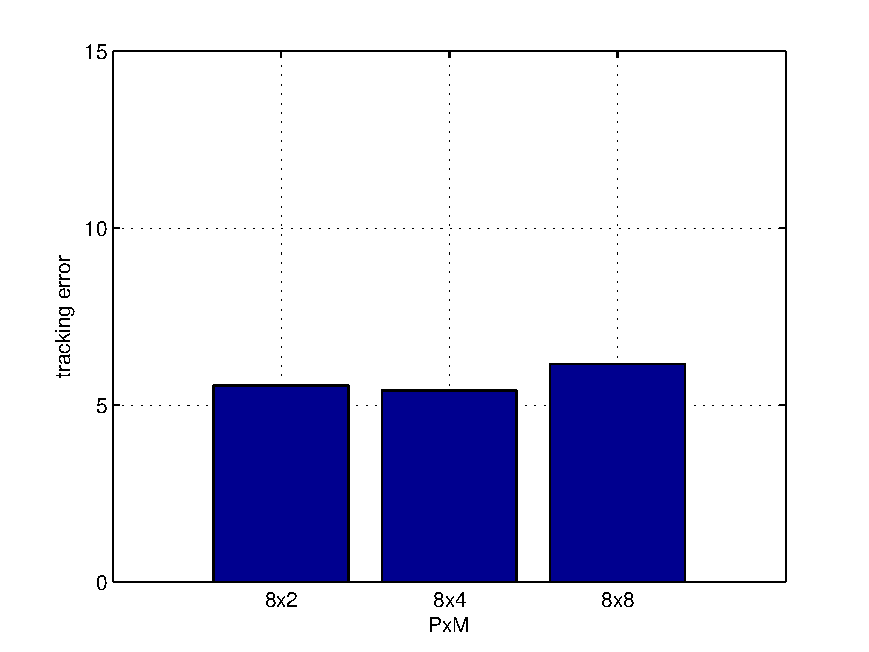
\includegraphics[width=0.3\textwidth]{thesis/results_final_5g_8x2_8x4_8x8.pdf}\label{fig:results_final_5g_8x2_8x4_8x8}}
								\caption{Tracking results (5 of 5), comparison of tracking performance as parameters for each algorithm are varied.  In (d), we see that over all RVQ algorithms, RofE has best mean performance.  In (g) it is clear that the best RVQ configuration is 8x4.}
								\label{fig:results_final_5_configs}
								\end{figure}

In this chapter, we present tracking error results for 6 different trackers, PCA-based, TSVQ-based and 4 RVQ-based trackers, maxP, RofE, nulE, and monR.  This chapter is organized as follows:

\begin{enumerate}
\item \underline{Datasets.}  We first present some details about the datasets used.
\item \underline{Results.}  Tracking results are presented in 5 figures, Figures~\ref{fig:results_final_1_best}, \ref{fig:results_final_2_mean}, \ref{fig:results_final_3_16}, \ref{fig:results_final_4_32} and~\ref{fig:results_final_5_configs}.  Our conclusions presented in the next chapter are based on the information presented in these 5 figures. These figures are derived from detailed experimental results for PCA, TSVQ, maxP, RofE, nulE and monR based tracking given in 6 figures, Figures~\ref{fig:results_final_pca_}, \ref{fig:results_final_tsvq}, \ref{fig:results_final_maxP}, \ref{fig:results_final_RofE} \ref{fig:results_final_nulE} and \ref{fig:results_final_monR} respectively in Appendix~\ref{App:tracking_error_plots}.   
\end{enumerate}

We begin by introducing the datasets we used in our work, and then present our results.

%====================================
\section{Datasets}
%====================================
All trackers were run on 6 publicly available datasets, Dudek, davidin300, sylv, fish, car4 and car11.  These datasets can be downloaded from~\cite{2008_JNL_subspaceTRK_Ross}.  See Figure~\ref{fig:trk_sequences} in Appendix~\ref{App:dataset_snapshots} for snapshots of images from each of these datasets at 100 frame intervals.  Tracking error was measured on each of these datasets using the error between ground truth feature points and estimated feature points as shown in Figure~\ref{fig:results_pca__trk_dudek_0007} for the Dudek sequence.

We begin by making some observations about each of these datasets.  This information is also presented in summarized form in Table~\ref{Tab:datasets_used}:

\begin{enumerate}
\item \underline{Dudek, davidin300}.  These sequences consist of indoors tracking of a human face through lighting, pose and expression changes with structured noise (putting on and taking off glasses).  In addition, the Dudek sequence has temporary occlusions and sudden motion.  These two sequences can be considered to be the most challenging datasets since they both have several different forms of noise.  A significant form of noise is blur due to sudden motion.  Additionally, these two sequences consist of tracking a face.  In related areas related to face processing, such as face recognition, it has been shown that 40 eigenfaces can be used to reconstruct a face with 3\% error~\cite{1987_JNL_Faces_Sirovich}.  However, performance levels off at about 25 principal components, or 45 principal components if the first 3 principal components are dropped~\cite{1997_JNL_EigenVsFisherFaces_Bel}.  The reason for dropping 3 principal components is that~\cite{1992_THE_GeoPhoto_Shashua} showed that for a fixed viewpoint, images of a Lambertian surface\footnote{A Lambertian surface, or informally a matte surface, is a surface that has constant BRDF (bidirectional reflectance distribution function).  BRDF has been explained earlier in the chapter.} under varying lighting conditions lie in a 3D linear subspace of the high-dimensional image space.  Although the first 3 principal components account for lighting changes in faces, these components are unlikely to only account for lighting variation and removing them may result in loss of important information~\cite{1997_JNL_EigenVsFisherFaces_Bel}.  Therefore, we do not remove any principal components in our PCA based tracker.  However, unlike the face recognition case, our tracking performance does not keep increasing till 20 or more eigenvectors.  The reason is that face alignment is noisy in tracking applications.  It appears that in these two sequences which have large pose changes, the first few eigenvectors are able to capture the linear dependencies in the slightly shifted faces.  After that, the later eigenvectors explain the residual noise.  This can lead to decreased tracking performance since reconstructions using an eigenspace that partially explains noise will be noisy.  Noisy reconstructions will get inaccurate DFFS (distance-from-feature-space) scores, which in turn will cause incorrect weighting for particle filter candidates in the tracking process.  This will lead to larger tracking error.
  
\item  \underline{Fish}.  This sequence consists of tracking a fish shaped wooden structure that is placed on a table.  In this indoors sequence, the lights are turned on and off resulting in large and abrupt lighting changes.  Moreover, the camera is shaken violently throughout the sequence.

\item  \underline{Sylv, car4 and car11}.  The sylv sequence consists of indoor tracking of a plush toy with some lighting variation and some pose changes.  The car4 and car11 sequences consist of outdoor tracking of vehicles during the day and night respectively.  The car4 sequence has one period of large lighting change when it moves under a bridge shadow.  The pose variation is gradual as the car changes lanes.  The car11 sequence also has less variation in lighting and pose as compared to some of the other sequences.
\end{enumerate}


%\begin{enumerate}
%\item \underline{Continually increasing error}.  For Dudek and sylv, the error continues to increase from $Q=8$ to $Q=32$.
%\item \underline{Sharply decreasing, then sharply increasing error}. For davidin300 and fish, the error decreases from $Q=8$ to $Q=16$, and then increases from $Q=16$ to $Q=32$.   The tracking error at $Q=16$ is significantly lower than for $Q=8$ and $Q=32$.
%\item \underline{Mildly decreasing, then mildly increasing error}.  For car4 and car11, like for davidin300 and fish above, the error decreases from $Q=8$ to $Q=16$, and then increases from $Q=16$ to $Q=32$.  However, the drop and rise in error is not as steep.
%\item \underline{Highest error}.  The average error for the Dudek sequence is highest.  This is because this sequence contains more variation than all other sequences including temporary occlusions, expression changes, structured noise, lighting changes and pose changes.  
%\item \underline{Face tracking}.  
%\end{enumerate}

We now present our results based on 5 metrics, best possible performance for each algorithm over all its parameters (Figure~\ref{fig:results_final_1_best}), mean performance for each algorithm (Figure~\ref{fig:results_final_2_mean}), tracking performance if only 16 (Figure~\ref{fig:results_final_3_16}) or 32 (Figure~\ref{fig:results_final_4_32}) eigenvectors or code-vectors are stored in memory, and finally, mean tracking performance over all datasets for each algorithm (Figure~\ref{fig:results_final_5_configs}). 


%===========================================
\section{Best performance}
%===========================================
We start with Figure~\ref{fig:results_final_1_best}.  In this figure, we plot best possible tracking performance for each algorithm.  For PCA, this means the best possible performance attained for each of the datasets for number of eigenvectors $Q$=8, 16 and 32.  For TSVQ, best possible performance for each dataset is over number of stages $P$=3, 4 and 5.  For maxP, RofE, nulE and monR, best possible performance for each dataset is over number of stages $P$ and number of codevectors $M$, $PxM$=8x2, 8x4 and 8x8.  The reason for plotting performance for each dataset separately is that each dataset represents a different distribution and we would like to gauge performance for each algorithm over the different distributions.  We see that performance for PCA and all 4 RVQ based algorithms is very close while TSVQ tracking error is highest in many cases.  

PCA performs best in the fish, car4 and car11 sequences while RVQ performs best in the remaining three datasets, Dudek, davidin300 and sylv.  TSVQ does not perform best in any sequence.  Note that the performance difference between PCA and RVQ in the car4 and car11 sequences is negligible.  Recall that car4 and car11 are relatively benign datasets with little variation in pose and lighting.  The fish sequence has sudden motion as well as sudden global lighting changes.   Since global lighting change induces linear correlation in the data, it makes sense that PCA does well in this sequence.  The reason is that global illumination changes move the illuminated object within the modeled PCA subspace~\cite{1987_JNL_Faces_Sirovich}.  %For a VQ based method such as RVQ or TSVQ, several codevectors would have to be dedicated to different lighting conditions to model all possible lighting changes.  

RVQ performs best over the Dudek, davidin300 and sylv sequences.  All 3 of these sequences have moderate lighting changes while Dudek and davidin300 have several forms of noise as discussed earlier.  For Dudek, RofE does best.  The reason is that in the presence of uncertainties, RofE holds tight to what has already been modeled and is resistant to accepting sudden changes in the underlying distribution.  It is therefore better able to handle blur and other forms of noise that do not exist in the training data.  On the other extreme is monR which greedily attempts to minimize reconstruction error.  Out of all RVQ methods, this method performs worse, but even then, not by much.  Second best performance is for maxP which is again not a greedy method.  Third best performance is for nulE which is also a greedy method but less so than monR.

%===========================================
\section{Mean performance over parameters}
%===========================================
We now turn to Figure~\ref{fig:results_final_2_mean}.  In this figure, mean performance over all parameters is shown.  It may be noted that monR loses track in one instance.  That instance is not factored into the means since it is not clear how penalize a lost track when performing mean computations.  Here, we see that RVQ performs best 66.7\% of the time.  This time, in addition to Dudek, davindin300 and sylv, RVQ performs better than PCA in the fish sequence as well.  The reason for this is that PCA is unable to track the fish sequence well when it has too few, i.e., 8 eigenvectors or when it has too many, i.e., 32 eigenvectors.  In the 8 eigenvector case, the subspace does not have enough dimensions to model lighting changes well.  Even though it has been shown, as mentioned earlier, that only 3 eigenvectors are needed to model lighting changes~\cite{1987_JNL_Faces_Sirovich}, in practice this does not hold due to shadowing and specularities~\cite{1997_JNL_EigenVsFisherFaces_Bel}.  For too many eigenvectors, over-fitting is an issue.  For $Q=16$, PCA performs best and that is why it had best possible performance.  However, when it comes to means, all 4 RVQ parameters are able to outperform PCA in mean performance.

%===========================================
\section{Memory = 16 vectors}
%===========================================
In Figure~\ref{fig:results_final_3_16}, we hold the number of eigenvectors for PCA or codevectors for TSVQ and RVQ constant at 16 (actually 14 for TSVQ but we ignore this slight difference).  In these figures, we see that PCA outperforms RVQ for 16 vectors.

%===========================================
\section{Memory = 32 vectors}
%===========================================
In Figure~\ref{fig:results_final_4_32}, we hold the number of eigenvectors for PCA or codevectors for TSVQ and RVQ constant at 32 (actually 30 for TSVQ but we ignore this slight difference).  In these figures, we see that RVQ completely outperforms PCA for 32 vectors.  The reason is that at $8x4$, RVQ now has enough capacity to explain the underlying distributions, and is better able to do so than PCA or TSVQ.


%===========================================
\section{Mean performance over datasets}
%===========================================
Finally, in Figure~\ref{fig:results_final_5_configs}, we plot mean tracking performance over all datasets for each algorithm.  Here we see that PCA performs best for $Q=16$, while both RofE and monR have best mean performance over all parameters and over all datasets.  Moreover, over all RVQ configurations, 8x4 performs best when averaged over all datasets.

In this figure, for 3 parameters per algorithm, $Q$=8, 16, 32 for PCA, $P$=3, 4, 5 for TSVQ and $PxM$ = 8x2, 8x4, 8x8 for RVQ, there are 4 possible outcomes listed below.  Of these, the first 3 are to be expected.  The fourth however requires further scrutiny.

\begin{enumerate}
\item \underline{Monotonically increasing error.}  This would mean that the degrees of freedom (DoF) in the learning algorithm, such as PCA, TSVQ or RVQ, model the underlying distribution well with low DoFs and adding DoFs is leading to over-training.  We do not see this performance in any case since we start with low DoFs for each algorithm.  We got an initial estimate of how many DoFs to use in our experiments on appearance modeling as shown in Figures~\ref{fig:PCA_results}, \ref{fig:RVQ_results_varyingP} \ref{fig:RVQ_results_varyingM} and \ref{fig:TSVQ_results}.
\item \underline{Monotonically decreasing error.}  This happens for TSVQ.  This means that adding more stages to TSVQ may increase performance and that TSVQ has not yet achieved optimum performance.  In our case, we use 3, 4 and 5 stages to keep the total number of stored code-vectors in TSVQ close to the stored code-vectors for RVQ and stored eigenvectors for PCA.  This also shows that PCA and RVQ are able to achieve optimum performance with less required memory storage than TSVQ.
\item \underline{Decreasing error followed by increasing error.}  We see this performance for PCA, maxP, nulE and monR.  This is a sign that the correct number of DoFs were chosen and that when error is minimum, the algorithm now has enough capacity to model the underlying distribution, but without over-fitting.
\item \underline{Increasing error followed by decreasing error.}  We see this in one case, RofE, and in some cases in TSVQ in Figure~\ref{fig:results_final_tsvq}.  To see this, consider the example of $K$=2, 4 and 8 code-vectors in $\mathbb{R}$ uniformly spaced on the inteval [0,7].  For $K$=2, the code-vectors are 2.33 and 4.66.  For the $K$=4 case, the code-vectors are 1.4, 2.8, 4.2 and 5.6.  For the $K$=8 case, the code-vectors are $\{0, 1, 2, 3, \ldots, 7\}$.  In regions around 2.33 and 4.6, there are certain contiguous regions where the reconstruction error is greatest for $K$=4.  This shows that although in general, one would not expect reconstruction error to be lowest for an intermediate number of code-vectors $K$, it is possible for a test vector to have highest reconstruction error for an intermediate $K$.  If such an error occurs during tracking, then in certain cases, it may not be possible to recover from this error.  See Figures~\ref{fig:results_TSVQ_Dudek_errors}, \ref{fig:results_TSVQ_Dudek_FN10} and \ref{fig:results_TSVQ_Dudek_FN457} in Appendix~\ref{App:TSVQ_Dudek_example} for an example of such a scenario for TSVQ while the target is moving quickly and the tracker is unable to recover from a single incorrect decision.  In learning based tracking, wrong decisions can be costly since there is no supervised learning mechanism to correct wrong labels.
\end{enumerate}

Having presented our results, we now present our conclusions in the next chapter.
%
%For PCA, on average, $Q=16$ produces the lowest tracking error.  On average, the tracking error decreases from $Q=8$ to $Q=16$, and then increases from $Q=16$ to $Q=32$.  It appears that the number of eigenvectors required to capture the linear correlation in these datasets is between 16 and 32, but closer to 16.   







%\begin{table}[h!]
%\centering
%\begin{tabular}{|l|c|c|c|}
\hline
&\textbf{PCA}&\textbf{TSVQ}&\textbf{RVQ}\\\hline
\textbf{Dudek}&7.44&8.62&6.68\\\hline
\textbf{davidin300}&4.60&5.93&4.29\\\hline
\textbf{sylv}&4.34&4.61&4.19\\\hline
\textbf{fish}&2.17&4.59&2.60\\\hline
\textbf{car4}&4.60&5.11&4.72\\\hline
\textbf{car11}&2.13&2.21&2.00\\\hline
\textbf{mean}&4.21&5.18&4.08\\\hline
\end{tabular}

%\caption{Comparison of best possible tracking error between PCA, RVQ and TSVQ over all algorithm parameters for 6 publicly available challenging datasets, Dudek, davidin300, sylv, fish, car4 and car11.  The table shows that RVQ produces the best results for 4 of the 6 datasets.  Overall tracking error is least for RVQ followed by PCA, and then followed by TSVQ.}
%\end{table}
%
%\begin{table}[h!]
%\centering
%\input{thesis/tables_comparison_DOF_16}
%\caption{Comparison of tracking results using the same DoF, 16 eigenvectors for PCA, 8x2 RVQ and 3x2 TSVQ (15 DOF for TSVQ, 8 terminal code-vectors and 7 stage code-vectors).  RVQ has best overall tracking performance.}
%\end{table}
%
%\begin{table}[h!]
%\centering
%\input{thesis/tables_comparison_DOF_32.tex}
%\caption{Comparison of tracking results using the same DoF, 32 eigenvectors for PCA, 8x4 RVQ and 4x2 TSVQ (31 DOF for TSVQ, 16 terminal code-vectors and 15 stage code-vectors).  RVQ has best tracking performance every time, and therefore also best overall performance.}
%\end{table}



%\end{Body}
%%##############################################################################################################
%\begin{EndMatter}
%\references 				%generates the bibliography page
%\end{EndMatter}
%\end{document}
%%##############################################################################################################
%
